\documentclass{article}\usepackage[]{graphicx}\usepackage[]{color}
%% maxwidth is the original width if it is less than linewidth
%% otherwise use linewidth (to make sure the graphics do not exceed the margin)
\makeatletter
\def\maxwidth{ %
  \ifdim\Gin@nat@width>\linewidth
    \linewidth
  \else
    \Gin@nat@width
  \fi
}
\makeatother

\definecolor{fgcolor}{rgb}{0.345, 0.345, 0.345}
\newcommand{\hlnum}[1]{\textcolor[rgb]{0.686,0.059,0.569}{#1}}%
\newcommand{\hlstr}[1]{\textcolor[rgb]{0.192,0.494,0.8}{#1}}%
\newcommand{\hlcom}[1]{\textcolor[rgb]{0.678,0.584,0.686}{\textit{#1}}}%
\newcommand{\hlopt}[1]{\textcolor[rgb]{0,0,0}{#1}}%
\newcommand{\hlstd}[1]{\textcolor[rgb]{0.345,0.345,0.345}{#1}}%
\newcommand{\hlkwa}[1]{\textcolor[rgb]{0.161,0.373,0.58}{\textbf{#1}}}%
\newcommand{\hlkwb}[1]{\textcolor[rgb]{0.69,0.353,0.396}{#1}}%
\newcommand{\hlkwc}[1]{\textcolor[rgb]{0.333,0.667,0.333}{#1}}%
\newcommand{\hlkwd}[1]{\textcolor[rgb]{0.737,0.353,0.396}{\textbf{#1}}}%
\let\hlipl\hlkwb

\usepackage{framed}
\makeatletter
\newenvironment{kframe}{%
 \def\at@end@of@kframe{}%
 \ifinner\ifhmode%
  \def\at@end@of@kframe{\end{minipage}}%
  \begin{minipage}{\columnwidth}%
 \fi\fi%
 \def\FrameCommand##1{\hskip\@totalleftmargin \hskip-\fboxsep
 \colorbox{shadecolor}{##1}\hskip-\fboxsep
     % There is no \\@totalrightmargin, so:
     \hskip-\linewidth \hskip-\@totalleftmargin \hskip\columnwidth}%
 \MakeFramed {\advance\hsize-\width
   \@totalleftmargin\z@ \linewidth\hsize
   \@setminipage}}%
 {\par\unskip\endMakeFramed%
 \at@end@of@kframe}
\makeatother

\definecolor{shadecolor}{rgb}{.97, .97, .97}
\definecolor{messagecolor}{rgb}{0, 0, 0}
\definecolor{warningcolor}{rgb}{1, 0, 1}
\definecolor{errorcolor}{rgb}{1, 0, 0}
\newenvironment{knitrout}{}{} % an empty environment to be redefined in TeX

\usepackage{alltt}

\usepackage{fancyhdr} % Required for custom headers
\usepackage{lastpage} % Required to determine the last page for the footer
\usepackage{extramarks} % Required for headers and footers
\usepackage{graphicx} % Required to insert images
\usepackage{hyperref}
\usepackage{amsmath} %for binomial pdf
\usepackage{parskip} % so that there's space bw paragraphs
\usepackage{float}
\usepackage{amsfonts}

% Margins
\topmargin=-0.45in
\evensidemargin=0in
\oddsidemargin=0in
\textwidth=6.5in
\textheight=9.0in
\headsep=0.25in 

\linespread{1.1} % Line spacing

% Set up the header and footer
\pagestyle{fancy}
\lhead{STAT 532: Bayes} % Top left header
\chead{Quiz 3} % Top center header
\rhead{Andrea Mack\\ Tan Tran\\ Moses Obiri} % Top right header
\lfoot{10/05/2016} % Bottom left footer
\cfoot{} % Bottom center footer
\rfoot{Page\ \thepage\ of\ \pageref{LastPage}} % Bottom right footer
\renewcommand\headrulewidth{0.4pt} % Size of the header rule
\renewcommand\footrulewidth{0.4pt} % Size of the footer rule

\setlength\parindent{0pt} % Removes all indentation from paragraphs
\setlength\parskip{0.5cm}
\restylefloat{table}

%----------------------------------------------------------------------------------------
%	DOCUMENT STRUCTURE COMMANDS
%	Skip this unless you know what you're doing
%----------------------------------------------------------------------------------------

% Header and footer for when a page split occurs within a problem environment
\newcommand{\enterProblemHeader}[1]{
\nobreak\extramarks{#1}{#1 continued on next page\ldots}\nobreak
\nobreak\extramarks{#1 (continued)}{#1 continued on next page\ldots}\nobreak
}

% Header and footer for when a page split occurs between problem environments
\newcommand{\exitProblemHeader}[1]{
\nobreak\extramarks{#1 (continued)}{#1 continued on next page\ldots}\nobreak
\nobreak\extramarks{#1}{}\nobreak
}


%----------------------------------------------------------------------------------------%
\IfFileExists{upquote.sty}{\usepackage{upquote}}{}
\begin{document}


\begin{enumerate}
\item%1 

\begin{knitrout}
\definecolor{shadecolor}{rgb}{0.969, 0.969, 0.969}\color{fgcolor}
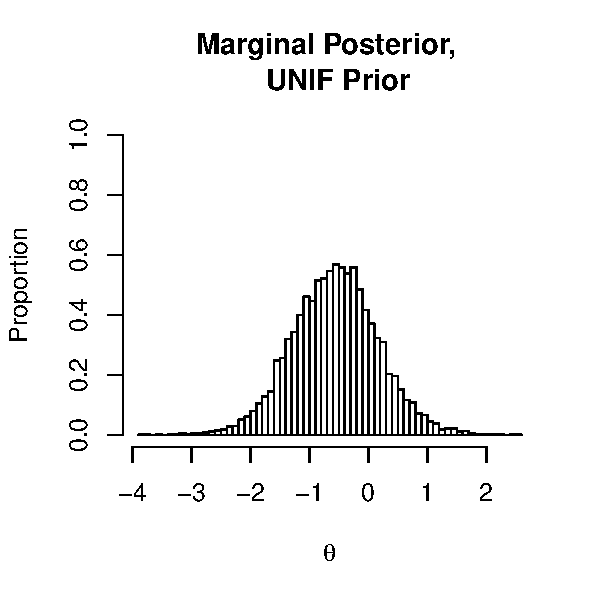
\includegraphics[width=\maxwidth]{figure/prob1-1} 

\end{knitrout}

\item %2


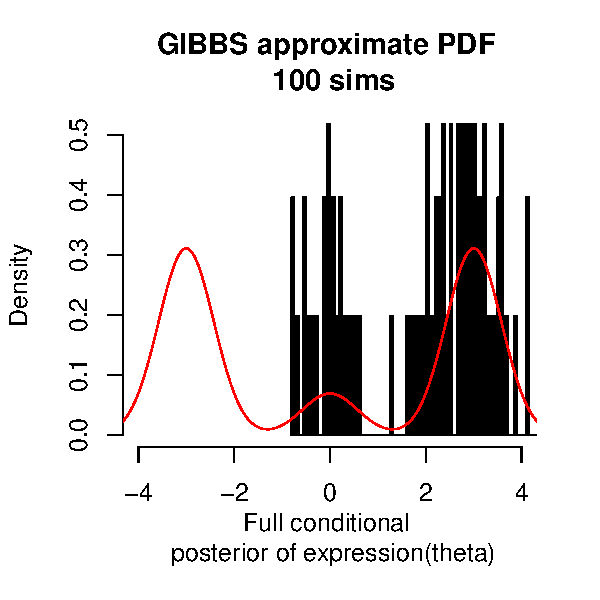
\includegraphics[width=\maxwidth]{figure/prob2-1} 

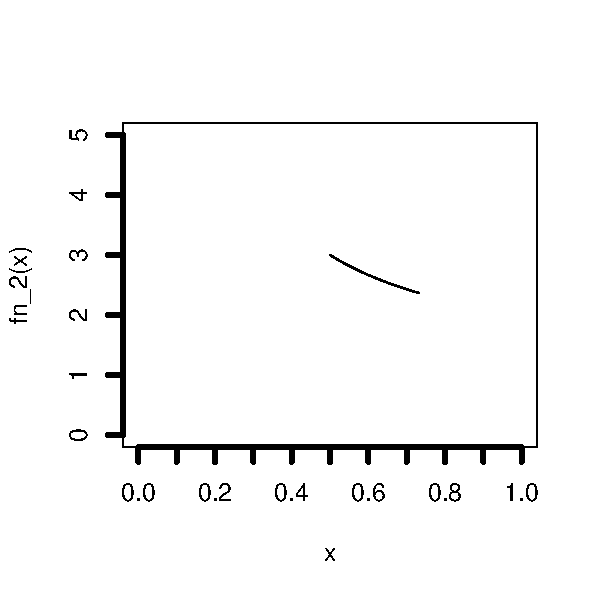
\includegraphics[width=\maxwidth]{figure/prob2-2} 


The trace plot shows that mixing begins after about 20 simulations, but does not include the part of the distribution centered at -3, also shown in the histogram.


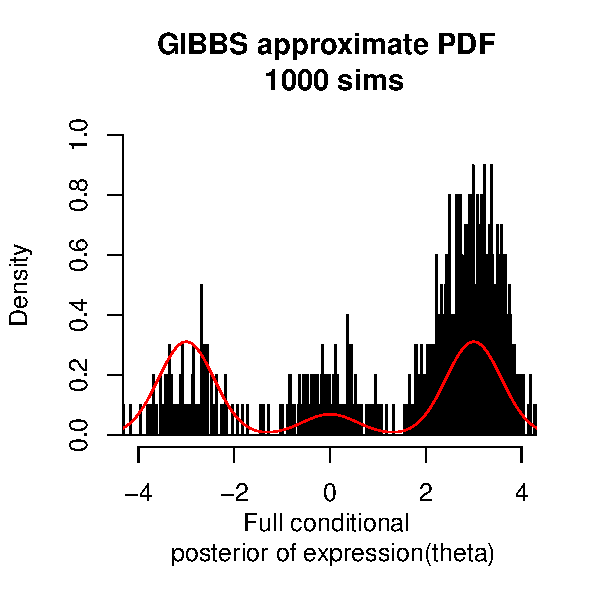
\includegraphics[width=\maxwidth]{figure/prob2e4-1} 

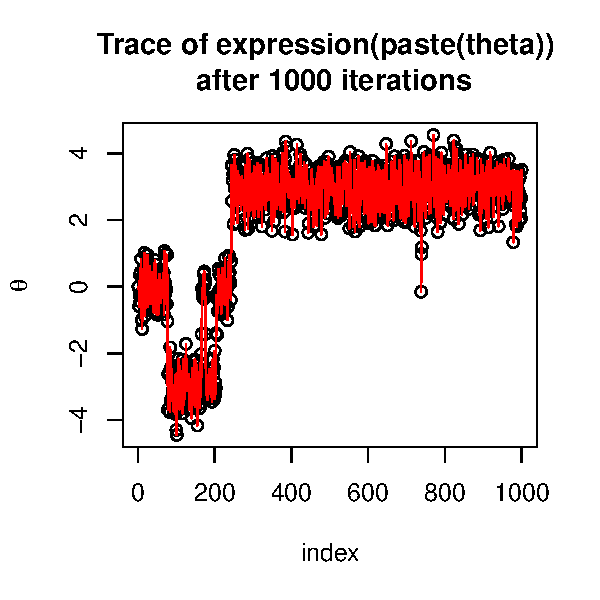
\includegraphics[width=\maxwidth]{figure/prob2e4-2} 


In the trace plot and histogram show most the observations around -3. With the larger number of simulations we would have hoped for more mixing.


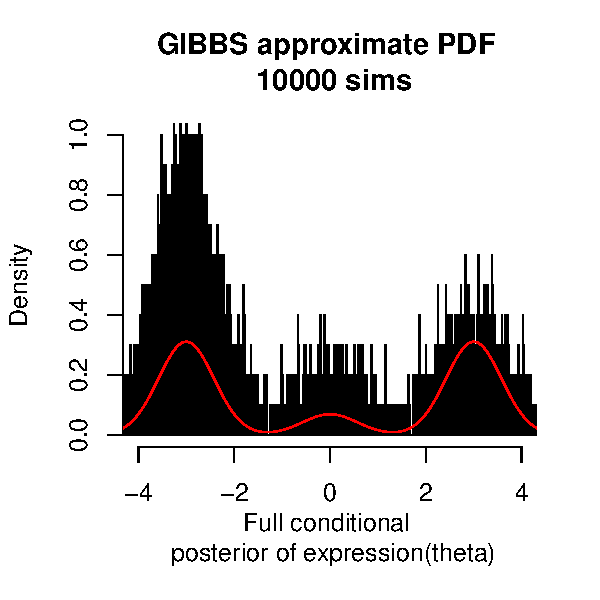
\includegraphics[width=\maxwidth]{figure/prob2e5-1} 

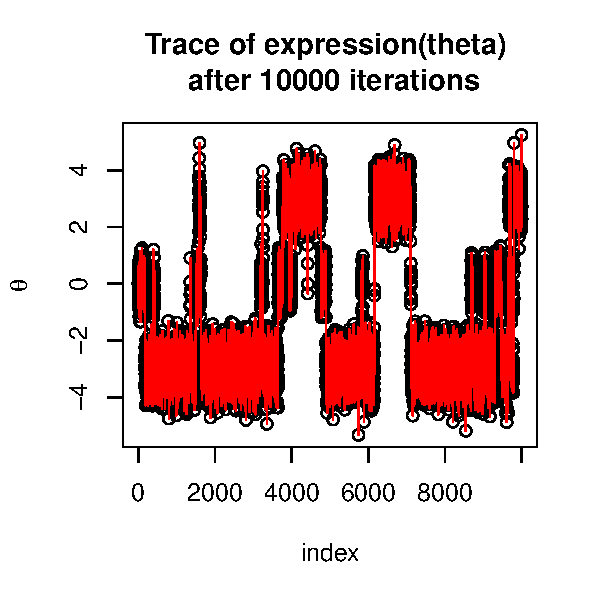
\includegraphics[width=\maxwidth]{figure/prob2e5-2} 


After 10000 simulations, the approximation appears to have converged, however the right portion of the plot still appears to be over sampled. Two thoughts: 

1) Is there a reason why the -3 region is always over sampled in each of these?

2) Could running more simulations may take us back out of convergence?


\item %3

Now the starting value for $\theta$ will be 100.

\begin{kframe}


{\ttfamily\noindent\bfseries\color{errorcolor}{\#\# Error in sample.int(length(x), size, replace, prob): NA in probability vector}}\end{kframe}
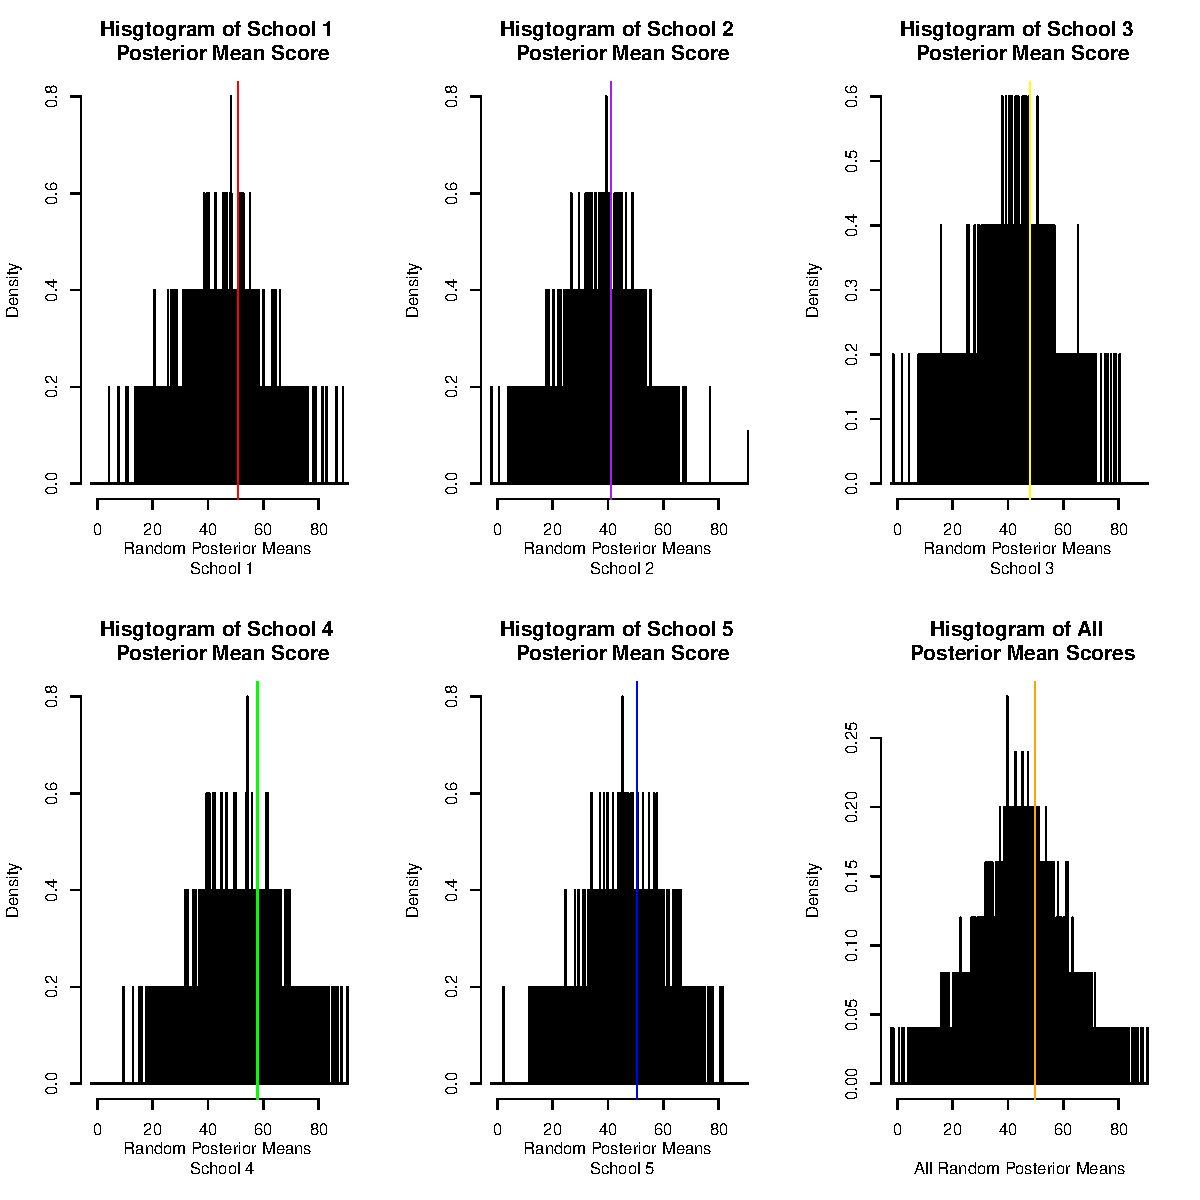
\includegraphics[width=\maxwidth]{figure/prob3-1} 

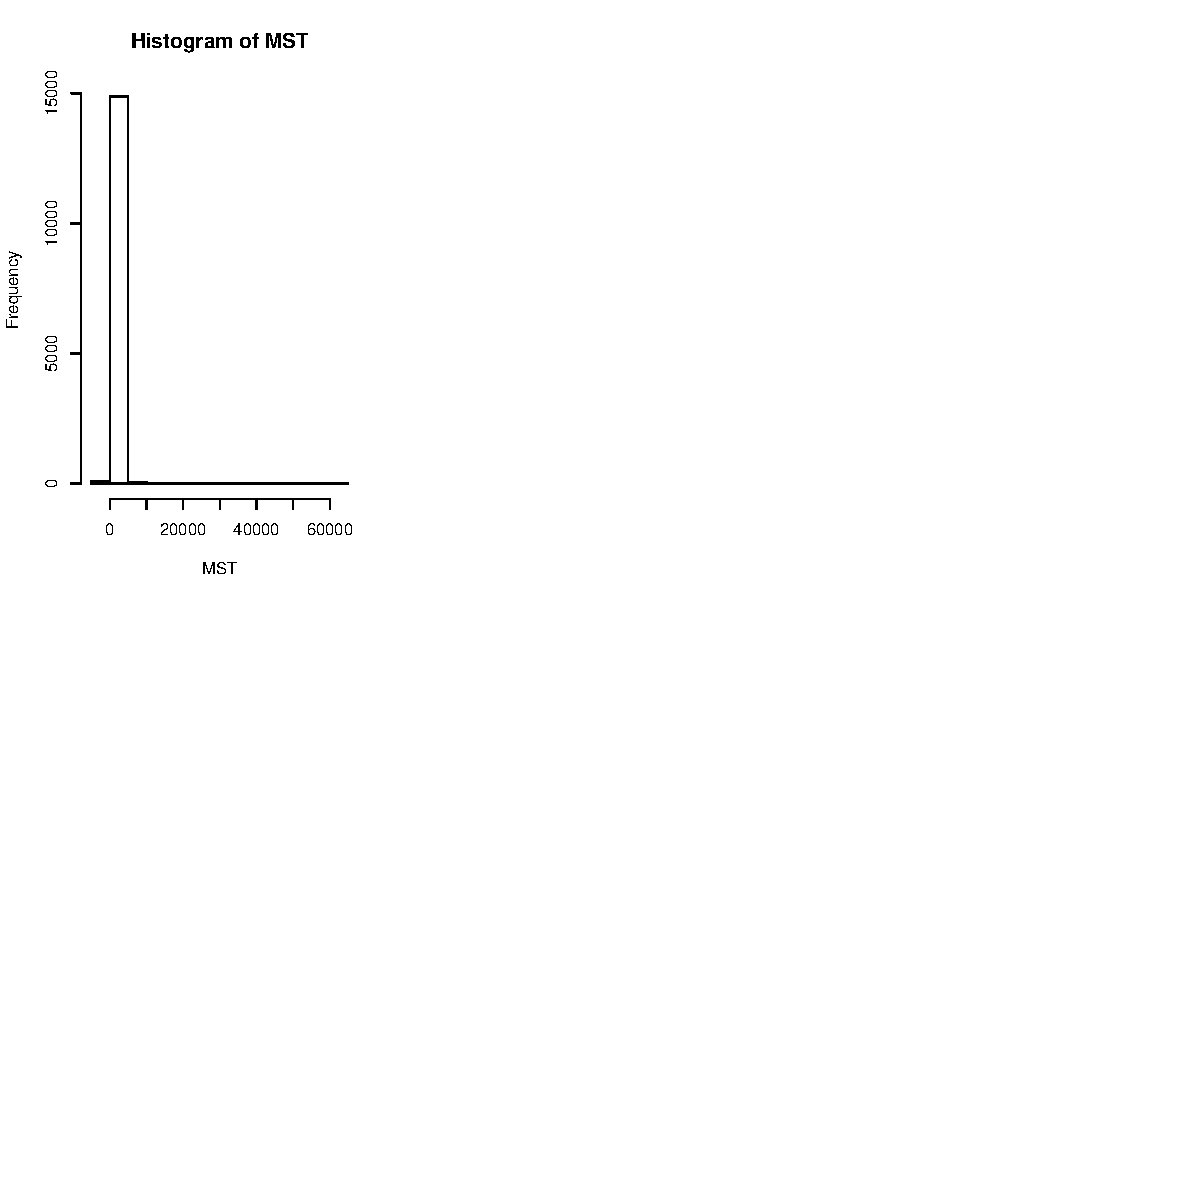
\includegraphics[width=\maxwidth]{figure/prob3-2} 


In 100 simulations, the -3 region of approximationss do not appear enough. The trace plot shows most of the approximations occur in a string, with values close to -3. Mixing first occurs after about 20 simulations. I did get an error about NA being in the probability vector. From the in class discussion, it seems that this appears because most of the mass of the distribution is below 5, the probability of $\theta$ being 100 is essentially 0, so when that is used to simulate the next value of $\sigma^2$, we are essentially dividing by 0, which results in the NA.



\begin{kframe}


{\ttfamily\noindent\bfseries\color{errorcolor}{\#\# Error in sample.int(length(x), size, replace, prob): NA in probability vector}}\end{kframe}
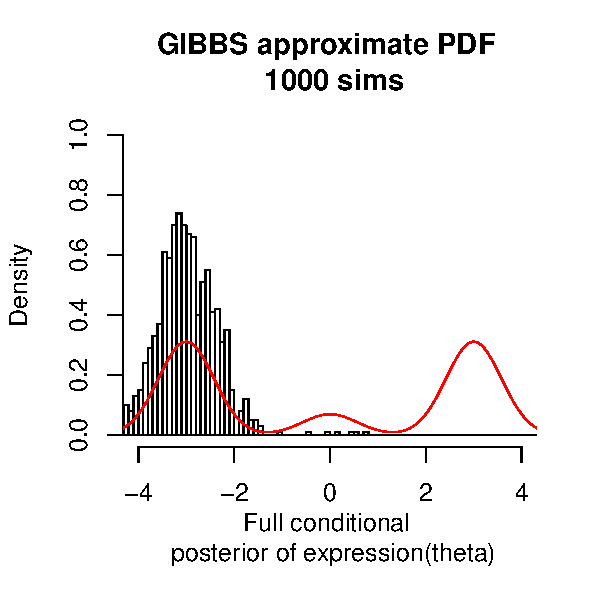
\includegraphics[width=\maxwidth]{figure/prob3e4-1} 

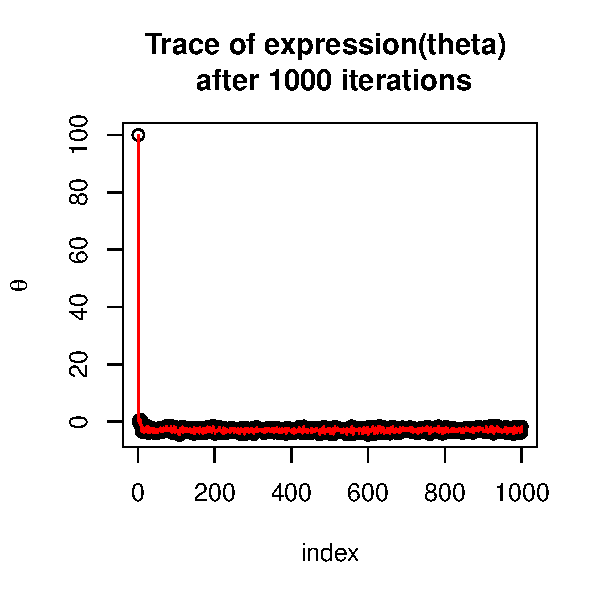
\includegraphics[width=\maxwidth]{figure/prob3e4-2} 


There is little mixing even with 1000 simulations and more are needed for convergence.

\begin{kframe}


{\ttfamily\noindent\bfseries\color{errorcolor}{\#\# Error in sample.int(length(x), size, replace, prob): NA in probability vector}}\end{kframe}
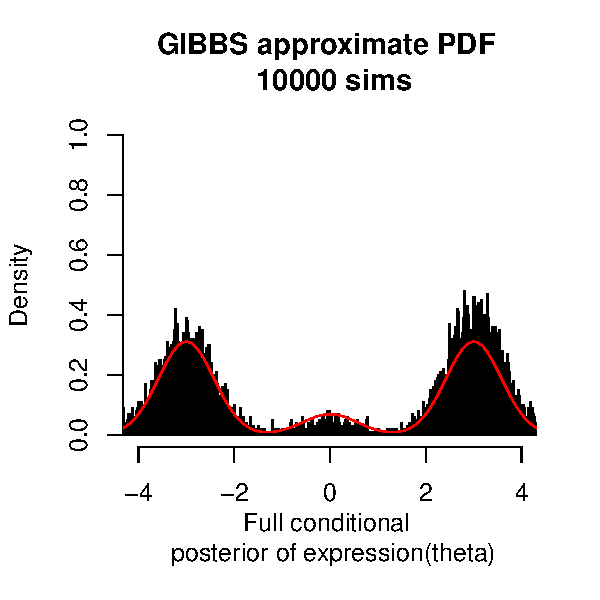
\includegraphics[width=\maxwidth]{figure/prob3e5-1} 

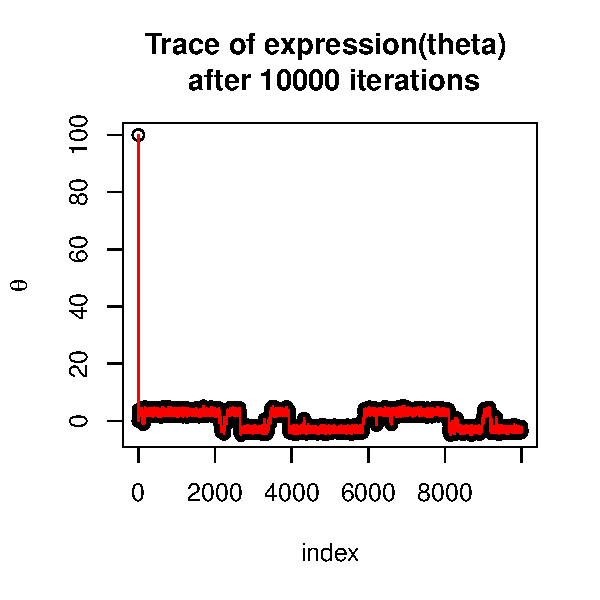
\includegraphics[width=\maxwidth]{figure/prob3e5-2} 


The trace plot for 10000 simulations here is interesting because a nice pattern in the approximated $\theta$'s doesn't appear until 4000 simulations, but then is fairly consistent up to 10000 simulations. Again, it would be interesting to know whether this is a property of Gibbs samplers, or whether the pattern eventually could break if we did enough simulations. 

It is nice that, in #3 compared to #2, it didn't matter that the starting value for $\theta$ was extremely large, it only took one simulation for it to be down in the expected range.

Comparing #2 and #3 after 10000 simulations, there appears to be more approximations in the -3 in #2 and more approximations in the 3 range in #3. I'm not sure if that is by chance or can be explained.

The chains with $\theta_{o}$ = 0 appear to be shorter than with $\theta_{o}$ = 100, which is most apparent in the 10000 simulations of each.



\end{enumerate}

\end{document}
